\subsection{InGame - Interface}

Das Modul InGame - Interface existiert um Daten asynchron zwischen SimulationsThread und RenderThread auszutauschen.
Es besteht aus einer Datenstruktur, welche in der Lage ist den Zustand aller dynamischen Objekte in der Szene eindeutig festzuhalten,
und einem Interpreter, welcher aus der Datenstruktur den Scenegraph konstruiert.
Die Datenstruktur und der Interpreter sind modular, somit lassen sich für dynamische Objekte beliebig viele verschiedene Eigenschaften definieren
und umsetzen.

\begin{figure}[htbp]
    \centering
    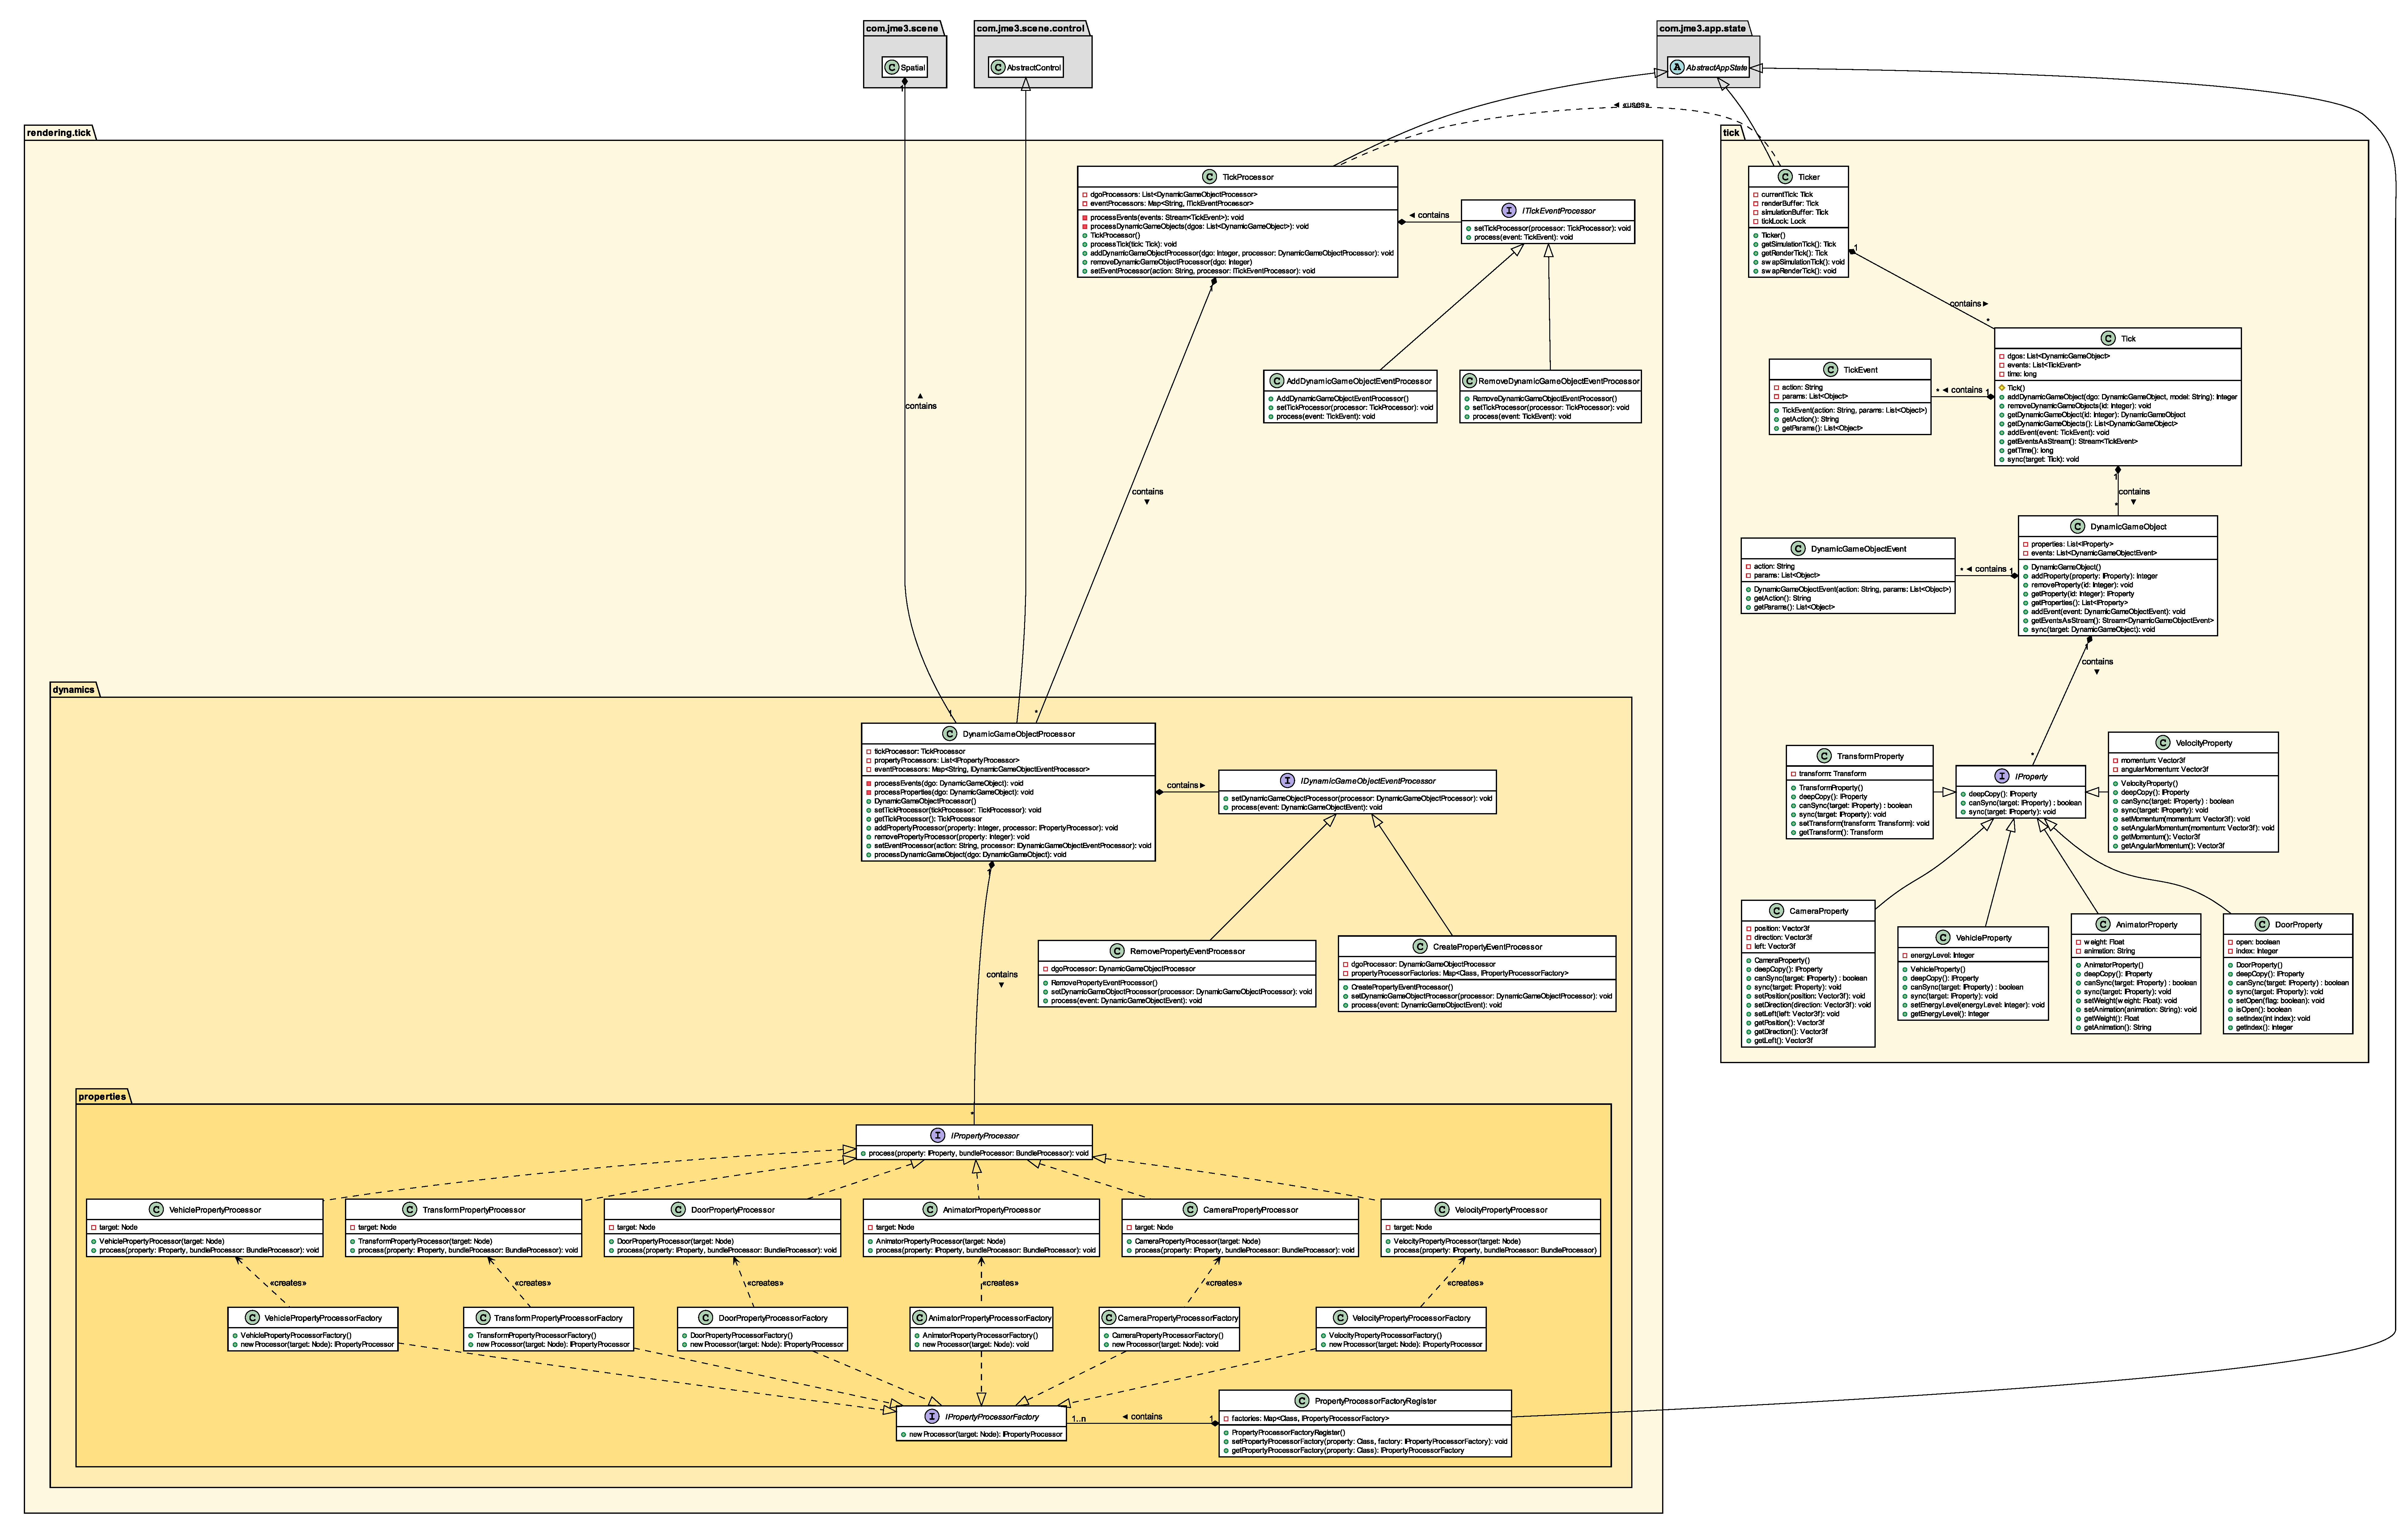
\includegraphics[width=\linewidth]{Interface/modul.eps}
    \caption{InGame - Interface Klassen-Diagram}
\end{figure}

\pagebreak